\chapter{Implementatie}

\section{Technologieën en software}

\subsection{TarsosDSP}

TarsosDSP is een Java bibliotheek voor realtime audio analyse en verwerking ontwikkeld aan het IPEM. De bibliotheek bevat een groot aantal algoritmes voor audioverwerking en kan nog verder worden uitgebreid. Deze bibliotheek wordt beschreven in artikel \cite{six2014tarsosdsp}. 

Een processing pipeline wordt voorgesteld als instantie van de klasse \texttt{AudioDispatcher}. Het aanmaken gebeurt met behulp van de klasse \texttt{AudioDispatcherFactory}. Deze bevat statische methodes om een \texttt{AudioDispatcher} aan te maken van een audiobestand, een \texttt{float} array of een microfoon. Aan de pipeline kunnen verschillende \texttt{AudioProcessor}s worden toegevoegd. Een \texttt{AudioProcessor} is een interface met de methodes \texttt{process} en \texttt{processingFinished}. De \texttt{process} methode heeft als enige parameter een \texttt{AudioEvent}. Dit object bevat een audio blok, voorgesteld als \texttt{float} array met waarden tussen -1.0 en 1.0. De grootte van dit blokje audio, en de mate van overlapping tussen de opeenvolgende blokjes audio is instelbaar. Verder bevat dit object nog andere metadata zoals onder meer een \textit{timestamp}.

Afhankelijk van de implementatie van de \texttt{process} methode kan de audiostroom op een bepaalde manier verwerkt, geanalyseerd of gewijzigd worden.

\subsection{Panako}

Panako is net zoals TarsosDSP een Java bibliotheek, door de zelfde auteurs ontwikkeld aan het IPEM. Panako bevat buiten implementaties van algoritmen ook enkele applicaties die hiervan gebruik maken.  Deze bibliotheek wordt beschreven in artikel \cite{six2014panako}.

Panako bevat een open-source implementatie van het accoustic fingerprinting algoritme beschreven in de paper van Avery Li-Chun Wang\cite{Wang2003a}. Dit algoritme is verder uitgebreid zodat audio waarbij de toonhoogte verhoogd of verlaagd is, of audio die sneller of trager is afgespeeld toch gedetecteerd kan worden.

De bibliotheek bevat verschillende applicaties die gebruik maken van dit algoritme. Zo is het mogelijk om de fingerprints van een geluidsfragment te bekijken, matches tussen verschillende geluidsfragmenten te visualiseren, en grafisch te experimenteren met de verschillende parameters.

Er is ook een applicatie beschikbaar om verschillende geluidsfragmenten te synchroniseren. Deze applicatie maakt behalve van het accoustic fingerprinting algoritme ook nog gebruik van het kruiscovariantie algoritme. 

Wanneer de latency tussen de verschillende audiofragmenten bepaald is, dan kan de applicatie een shell script genereren dat met behulp van \textit{FFmpeg} stukjes van de geluidsbestanden wegknipt of er stilte aan toevoegt. Het resultaat is dat na het uitvoeren van het script de geluidsbestanden gesynchroniseerd zijn.

\subsection{FFmpeg}

FFmpeg is een command-line multimedia framework dat gebruikt wordt voor encoderen, decoderen, multiplexen, demultiplexen, streamen en afspelen van audio en video. \cite{kollarconfiguration}

In dit onderzoek wordt FFmpeg voornamelijk gebruikt in scripts bij het geautomatiseerd genereren van testdata.

\subsection{SoX}

SoX is net zoals FFmeg een command-line tool voor audioverwerking. Buiten de mogelijkheid om audiobestanden te converteren laat SoX ook minder triviale operaties toe. Zo is het onder meer mogelijk om het volume aan te passen, effecten toe te voegen, de bestanden bij te knippen of gegenereerde geluiden in een audiobestand te mixen.
\cite{barras2012sox}

In dit onderzoek wordt SoX ook gebruikt in scripts bij het manipuleren van de testdata.

\subsection{Sonic Visualiser}

\begin{figure}[!h]
	\captionsetup{width=0.7\textwidth}
	\caption[Gebruikersinterface van Sonic Visualiser]{De gebruikersinterface van Sonic Visualiser}
	\advance\parskip0.3cm
	\centering
	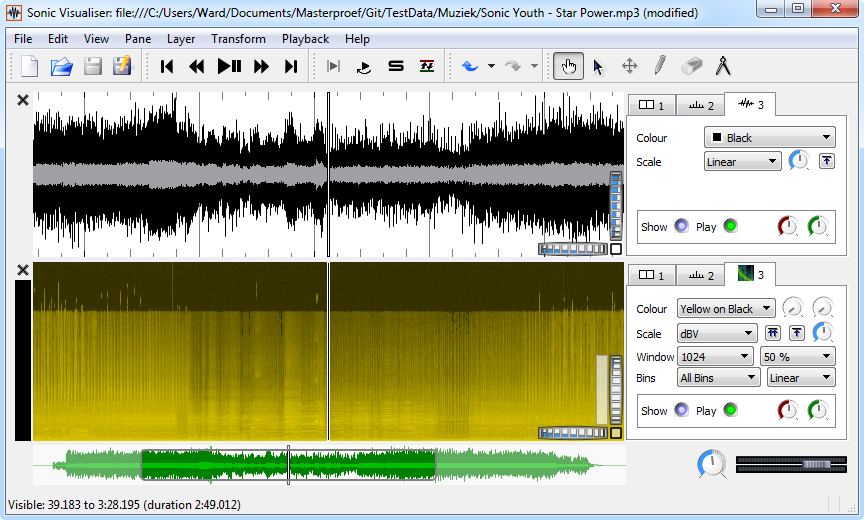
\includegraphics[width=0.7\textwidth]{sonicvisualiser.png}
\end{figure}

Sonic Visualiser is een gebruiksvriendelijke desktopapplicatie voor de analyse, visualisatie van audiobestanden. Sonic Visualiser laat toe om audiobestanden vanuit verschillende perspectieven te analyseren, zo kan zowel de waveform als het spectrogram van een audiobestand gevisualiseerd worden. Sonic Visualiser is uitbreidbaar met plug-ins in het Vamp formaat. \cite{cannam2010sonic}

Sonic visualiser is in dit onderzoek gebruikt om handmatig de latency tussen verschillende audiofragmenten te bepalen. De applicatie is ook gebruikt geweest om de principes achter de algoritmes te visualiseren. 

\subsection{Audacity}

\begin{figure}[!h]
	\captionsetup{width=0.7\textwidth}
	\caption[Gebruikersinterface van Audacity]{De gebruikersinterface van Audacity}
	\centering
	\advance\parskip0.3cm
	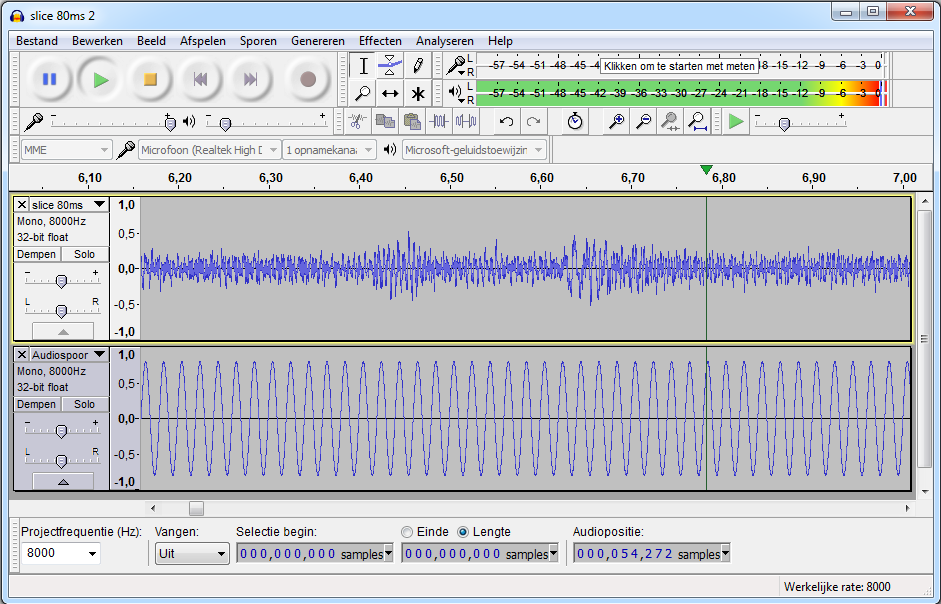
\includegraphics[width=0.7\textwidth]{audacity.png}
\end{figure}

Audacity is een open-source desktopapplicatie voor het bewerken, opnemen en converteren van audio. Met Audacity is het ook mogelijk om tal van effecten en filters aan audio toe te voegen.\cite{audacity2016}

Alle opnames en handmatige bewerkingen op audiobestanden in dit onderzoek zijn uitgevoerd met Audacity.


\subsection{Max/MSP}

\begin{figure}[!h]
	\captionsetup{width=0.7\textwidth}
	\caption[Gebruikersinterface van MAX/MSP]{De gebruikersinterface van MAX/MSP: een \textit{patch panel} met daarop enkele modules die met elkaar zijn verbonden.}
	\centering
	\advance\parskip0.3cm
	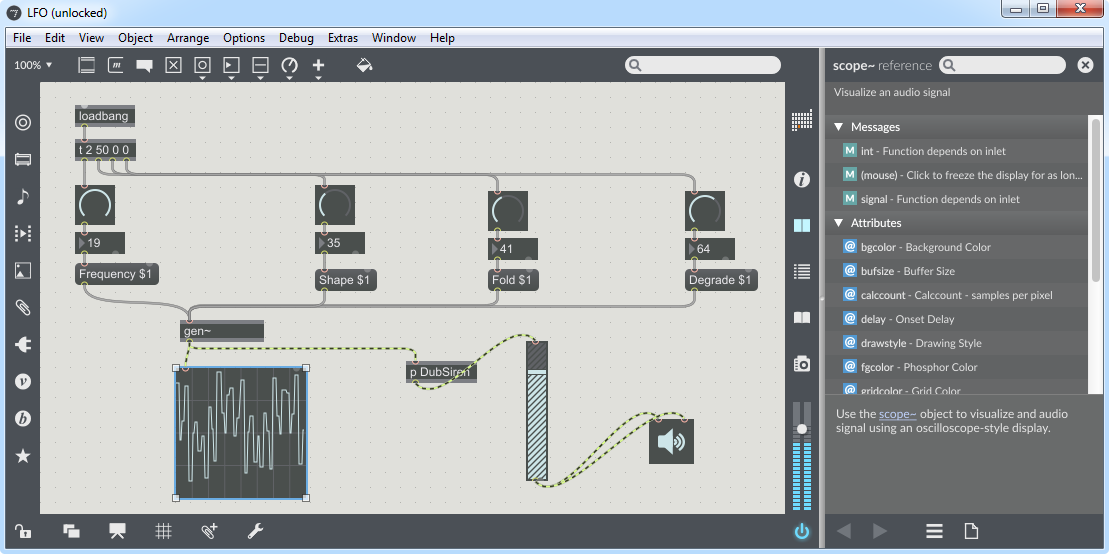
\includegraphics[width=0.7\textwidth]{maxmsp.png}
\end{figure}

Max/MSP is een visuele programmeertaal voor muziek en multimedia. Het is een systeem waarbij modules met elkaar verbonden kunnen worden om zo complexe systemen op te bouwen. Max/MSP beschikt ook over een API waarmee nieuwe modules mee ontwikkeld kunnen worden. \cite{cycling2016}

Max/MSP kan realtime audio verwerken, daarom zullen we deze toepassing gebruiken voor het ontwikkelen van onze gebruikersinterface. 

\subsection{Teensy}

\begin{figure}[!h]
	\captionsetup{width=0.7\textwidth}
	\caption[Teensy microcontroller]{De Teensy microcontroller verbonden met een infraroodsensor en microfoon op een breadboard.}
	\centering
	\advance\parskip0.3cm
	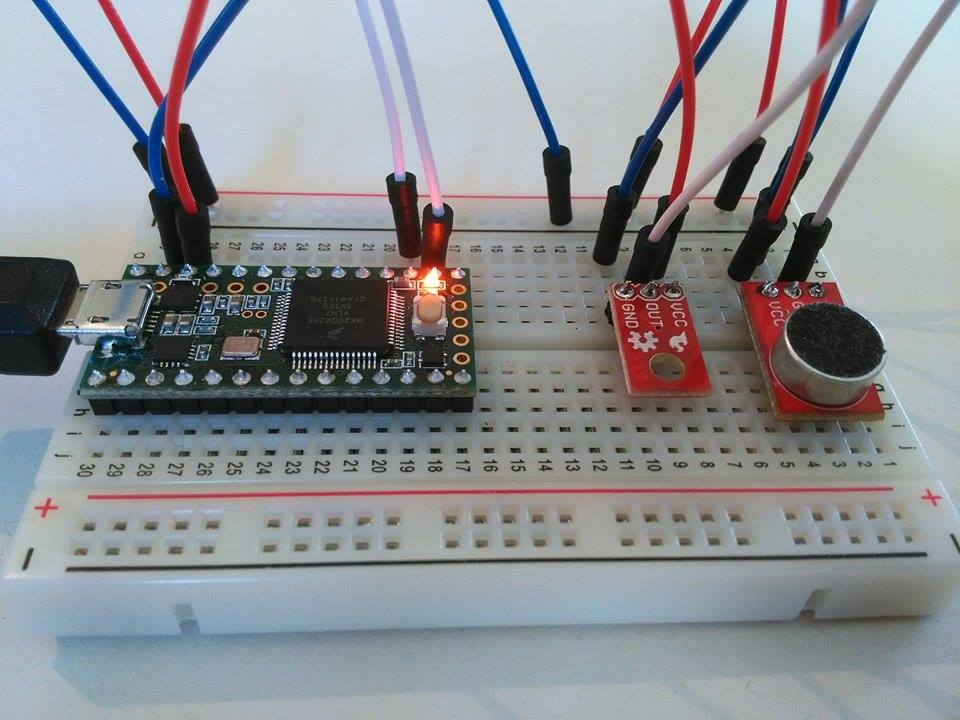
\includegraphics[width=0.4\textwidth]{teensy.jpg}
\end{figure}

De Teensy is een kleine microcontroller die via USB geprogrammeerd kan worden. De Teensy is compatibel met de Arduino software en is hierdoor zeer gebruiksvriendelijk. \cite{teensy2016}

De sensoren die gebruikt worden bij de experimenten van het IPEM zijn meestal aangesloten op Teensy microcontrollers.
Om de synchronisatiealgoritmes en het bijhorende systeem in een representatieve situatie te testen zal daarom ook gebruik gemaakt worden van een Teensy microcontroller.

In hoofdstuk \ref{evaluatie} wordt deze testopstelling meer in detail besproken.


\section{Algoritmen}

\subsection{Accoustic fingerprinting}

De Panako softwarebibliotheek bevat een zeer goede implementatie van het accoustic fingerprinting algoritme. Om wijzigingen mogelijk te maken hebben we de code van het algoritme overgenomen in ons eigen project. Deze code is wel nog steeds afhankelijk van enkele klassen uit het Panako project. 

\subsubsection{Optimalisaties}

Aan dit algoritme is één vereenvoudiging aangebracht. Het originele algoritme bevatte namelijk de mogelijkheid om alle offsets boven een bepaalde drempelwaarde te verwerken. Deze feature laat toe dat er meerdere matches kunnen gevonden worden binnen één uitvoering van het algoritme. Om dit te ondersteunen moeten alle matches echter wel één voor één worden vergeleken met de drempelwaarde. Omdat we in onze toepassing enkel geïnteresseerd zijn in de beste offsetwaarde is dit overbodig. De beste offset en bijhorende fingerprints wordt apart bijgehouden. De naverwerking wordt hierdoor vermeden.

\subsubsection{Parameters en hun invloed op het algoritme}
\label{accoustic-fingerprinting-params}

De werking van dit algoritme is afhankelijk van een aantal parameters die een grote invloed kunnen hebben op de performantie en de nauwkeurigheid van het uiteindelijke resultaat. Daarom is het van belang om voor het uitvoeren van het algoritme de waarde van deze parameters te controleren. De optimale waarde van elke parameter is afhankelijk van verschillende factoren die van situatie tot situatie kunnen verschillen:

\begin{itemize}[noitemsep]
\item De vereiste nauwkeurigheid van het algoritme.
\item De vereiste performantie van het algoritme.
\item De mate waarin er omgevingsgeluid aanwezig is.
\item De opnamekwaliteit van het omgevingsgeluid.
\end{itemize}

De meeste parameters worden bijgehouden in een configuratiebestand waardoor ze ook na compilatie wijzigbaar zijn. Dit zijn de belangrijkste parameters uit het configuratiebestand die invloed hebben op het algoritme:

\begin{description}
\item[\texttt{SAMPLE\_RATE}] \hfill \\
Deze parameter bepaalt de samplefrequentie van de binnenkomende audiostreams. Het verhogen van deze parameter zorgt voor een tragere verwerking maar een betere nauwkeurigheid.
\item[\texttt{NFFT\_BUFFER\_SIZE}] \hfill \\
Het FFT algoritme waarmee het spectrogram gegenereerd wordt maakt gebruik van een verschuivende buffer. De frequentiesterktes op een bepaalde plaats op de tijd\-as worden berekend per buffer. De grootte van deze buffer wordt bepaald door deze parameter.
\item[\texttt{NFFT\_STEP\_SIZE}] \hfill \\
Deze parameter stelt het aantal samples in van elke verschuiving in het FFT algoritme. Deze parameter beïnvloedt rechtstreeks de nauwkeurigheid van het accoustic fingerprinting algoritme. Wanneer deze parameter is ingesteld op 128 samples en de samplefrequentie 8000hz bedraagt dan is de maximale nauwkeurigheid $128/8000Hz = 0.016s = 16ms$.
\item[\texttt{MIN\_ALIGNED\_MATCHES}] \hfill \\
Een match tussen twee audiofragmenten wordt pas als geldig beschouwd wanneer er een bepaald aantal fingerprint matches met dezelfde offset gevonden zijn. Dit aantal wordt bepaalt door deze parameter.
\item[\texttt{NFFT\_MAX\_FINGERPRINTS\_PER\_EVENT\_POINT}] \hfill \\
Deze parameter bepaalt het maximum aantal fingerprints waaraan een event point (een punt op het spectrogram) kan deelnemen. Hoe hoger deze parameter hoe vlugger er matches kunnen gevonden worden. Wanneer \texttt{MIN\_ALIGNED\_MATCHES} hierbij niet wordt aangepast stijgt de kans op false positives. Bij een hoge waarde moeten meer berekeningen worden uitgevoerd, dit heeft invloed op de performantie.
\item[\texttt{NFFT\_EVENT\_POINT\_MIN\_DISTANCE}] \hfill \\
Dit is de minimale afstand tussen twee event points op het spectrogram die samen een fingerprint kunnen vormen. Omdat deze parameter een afstand uitdrukt in het tijd-frequentie domein is de eenheid ervan cent-seconde. Seconde is de eenheid van de waarden op de tijdas. Cent\footnote{Cent is een relatieve logaritmische eenheid waarmee het verschil tussen twee frequenties wordt uitgedrukt. Een belangrijke eigenschap van deze eenheid is dat de waarden als muzikale intervallen benaderd kunnen. Ze kunnen zonder problemen bij elkaar worden opgeteld of van elkaar worden afgetrokken en behouden hierbij hun betekenis. Het frequentieverschil in cent kan men als volgt berekenen:\\ 
\begin{math}
c = 1200 \times \log_{2}(\frac{f_{1}}{f_{2}})
\end{math} \cite{pitchrepresentation}} 
is de eenheid van het verschil in frequentie tussen de twee event points. 

\end{description}

Verder maakt het algoritme nog gebruik van twee hardgecodeerde parameters die niet instelbaar zijn in het configuratiebestand: \texttt{MIN\_FREQUENCY} en \texttt{MAX\_FREQUENCY}. Deze parameters bepalen binnen welke frequentiebereik er naar fingerprints gezocht worden. De waarden waarop deze ingesteld staan bevinden zich op de rand van de frequenties die door muziek of stemgeluid geproduceerd worden.

\subsubsection{Optimale instellingen}

%TODO optimale instellingen
\textit{De optimale instellingen van de parameters bespreken. Uitleggen waarom ze zo extreem zijn en waarom dit eigenlijk geen kwaad kan...}

\subsection{Kruiscovariantie}

%Lorem ipsum dolor sit amet, consectetur adipiscing elit. Maecenas at facilisis diam, vel varius mi. Maecenas in sodales tellus. Aenean tincidunt erat sit amet accumsan bibendum. Aliquam posuere dictum diam in tempor. Aenean feugiat eget quam id malesuada. Proin pretium et urna mattis molestie. Mauris pretium neque id magna sodales pulvinar. Cum sociis natoque penatibus et magnis dis parturient montes, nascetur ridiculus mus. Sed vel ornare leo. Nullam porttitor diam eget blandit hendrerit.

\subsubsection{Werking}

%Lorem ipsum dolor sit amet, consectetur adipiscing elit. Maecenas at facilisis diam, vel varius mi. Maecenas in sodales tellus. Aenean tincidunt erat sit amet accumsan bibendum. Aliquam posuere dictum diam in tempor. Aenean feugiat eget quam id malesuada. Proin pretium et urna mattis molestie. Mauris pretium neque id magna sodales pulvinar. Cum sociis natoque penatibus et magnis dis parturient montes, nascetur ridiculus mus. Sed vel ornare leo. Nullam porttitor diam eget blandit hendrerit.


\subsubsection{Optimalisaties}

%Bugfixes: onderschatten en overschatten van fingerprint maakt verschil
%Verschillende keren per slice uitvoeren, threshold
%Bandpass filtering die toch niet geïmplementeerd is.

%Lorem ipsum dolor sit amet, consectetur adipiscing elit. Maecenas at facilisis diam, vel varius mi. Maecenas in sodales tellus. Aenean tincidunt erat sit amet accumsan bibendum. Aliquam posuere dictum diam in tempor. Aenean feugiat eget quam id malesuada. Proin pretium et urna mattis molestie. Mauris pretium neque id magna sodales pulvinar. Cum sociis natoque penatibus et magnis dis parturient montes, nascetur ridiculus mus. Sed vel ornare leo. Nullam porttitor diam eget blandit hendrerit.

\subsubsection{Parameters en hun invloed op het algoritme}

%Lorem ipsum dolor sit amet, consectetur adipiscing elit. Maecenas at facilisis diam, vel varius mi. Maecenas in sodales tellus. Aenean tincidunt erat sit amet accumsan bibendum. Aliquam posuere dictum diam in tempor. Aenean feugiat eget quam id malesuada. Proin pretium et urna mattis molestie. Mauris pretium neque id magna sodales pulvinar. Cum sociis natoque penatibus et magnis dis parturient montes, nascetur ridiculus mus. Sed vel ornare leo. Nullam porttitor diam eget blandit hendrerit.

\subsection{Structuur softwarebibliotheek}

%De Java bibliotheek die verantwoordelijk is voor de realtime synchronisatie van de audiostromen heeft verschillende taken. Eerst en vooral moet de gestreamde data gebufferd worden, het is namelijk onmogelijk om de synchronisatiealgoritmes uit te voeren zonder dat er enkele seconden audio van elke stream zich in het geheugen bevind. Deze verantwoordelijkheid wordt afgehandeld in het \textit{slicer}-gedeelte van de bibliotheek. Wanneer de audio gebufferd is kan het synchronisatie-deel van de applicatie een synchronisatiealgoritme aanroepen en het geretourneerde resultaat teruggeven aan de gebruiker, of de aanroepende applicatie. Welk algoritme precies gebruikt wordt, en de specifieke parameters ervan, is configureerbaar met behulp van een configuratiebestand.

\subsection{Implementatie van een Max/MSP module}

%Gans dit onderzoek heeft uiteindelijk de bedoeling te resulteren in het ontwerp en implementatie van een module in MAX/MSP\footnote{Cycling ‘74 Max/MSP is een softwarepakket en een visuele programmeertaal waarmee audio, video en multimedia kan worden verwerkt met behulp van onafhankelijke modules. Deze modules kunnen met elkaar worden verbonden om zo complexe zaken te bereiken. Buiten de standaard meegeleverde modules is het ook mogelijk om zelf modules te schrijven.\cite{maxmsp2016}} die realtime synchronisatie mogelijk moet maken via een interface die bruikbaar is voor musicologen/onderzoekers met een beperkte informatica achtergrond.

%Deze module moet in staat zijn om verschillende datastromen als input binnen te krijgen, de synchronisatiebibliotheek aan te roepen, en de gesynchroniseerde datastromen als output terug te geven. Een andere Max module kan er dan voor zorgen dat deze data wordt weggeschreven naar een WAVE-bestand.